%%
%% This is file `sample-sigconf.tex',
%% generated with the docstrip utility.
%%
%% The original source files were:
%%
%% samples.dtx  (with options: `sigconf')
%% 
%% IMPORTANT NOTICE:
%% 
%% For the copyright see the source file.
%% 
%% Any modified versions of this file must be renamed
%% with new filenames distinct from sample-sigconf.tex.
%% 
%% For distribution of the original source see the terms
%% for copying and modification in the file samples.dtx.
%% 
%% This generated file may be distributed as long as the
%% original source files, as listed above, are part of the
%% same distribution. (The sources need not necessarily be
%% in the same archive or directory.)
%%
%% The first command in your LaTeX source must be the \documentclass command.

\documentclass[sigconf]{acmart}
\usepackage{bm}
\usepackage{array}
%%
%% \BibTeX command to typeset BibTeX logo in the docs
\AtBeginDocument{%
  \providecommand\BibTeX{{%
    \normalfont B\kern-0.5em{\scshape i\kern-0.25em b}\kern-0.8em\TeX}}}

%% Rights management information.  This information is sent to you
%% when you complete the rights form.  These commands have SAMPLE
%% values in them; it is your responsibility as an author to replace
%% the commands and values with those provided to you when you
%% complete the rights form.
\setcopyright{acmcopyright}
\copyrightyear{2020}
\acmYear{2020}
\acmDOI{10.1145/1122445.1122456}

%% These commands are for a PROCEEDINGS abstract or paper.
\acmConference[SBES '20]{SBES '2020: XXXIV BRAZILIAN SYMPOSIUM ON SOFTWARE ENGINEERING (SBES 2020)}{October 19--23, 2020}{Natal, Brazil}
\acmBooktitle{XXXIV BRAZILIAN SYMPOSIUM ON
SOFTWARE ENGINEERING (SBES 2020),
  October 19--23, 2020, Natal, Brazil}


%%
%% Submission ID.
%% Use this when submitting an article to a sponsored event. You'll
%% receive a unique submission ID from the organizers
%% of the event, and this ID should be used as the parameter to this command.
%%\acmSubmissionID{123-A56-BU3}

%%
%% The majority of ACM publications use numbered citations and
%% references.  The command \citestyle{authoryear} switches to the
%% "author year" style.
%%
%% If you are preparing content for an event
%% sponsored by ACM SIGGRAPH, you must use the "author year" style of
%% citations and references.
%% Uncommenting
%% the next command will enable that style.
%%\citestyle{acmauthoryear}

%%
%% end of the preamble, start of the body of the document source.
\begin{document}

%%
%% The "title" command has an optional parameter,
%% allowing the author to define a "short title" to be used in page headers.
\title{CoNCRA: A Convolutional Network Code Retrieval Approach}

%%
%% The "author" command and its associated commands are used to define
%% the authors and their affiliations.
%% Of note is the shared affiliation of the first two authors, and the
%% "authornote" and "authornotemark" commands
%% used to denote shared contribution to the research.
\author{Marcelo de Rezende Martins}
\email{rezende.martins@gmail.com}
\affiliation{%
  \institution{IPT – Institute for Technological Research}
  \city{Sao Paulo}
  \state{Sao Paulo}
  \country{Brazil}
}


\author{Marco Aurélio Gerosa}
\email{marco.gerosa@nau.edu}
\affiliation{%
  \institution{Northern Arizona University (NAU)}
  \city{Flagstaff}
  \state{Arizona}
  \country{United States}
}

%%
%% By default, the full list of authors will be used in the page
%% headers. Often, this list is too long, and will overlap
%% other information printed in the page headers. This command allows
%% the author to define a more concise list
%% of authors' names for this purpose.


%%
%% The abstract is a short summary of the work to be presented in the
%% article.
\begin{abstract}
   Code search is a prevalent task in software development process. According to \cite{what-developers-search-for-on-the-web:xia:2017}, developers spend 15\% of their time searching for API's examples, what a code does and how to fix a bug. A research at Google showed that developers search for code 12 times a day, checking 2 and 3 results per search session. Most of the time, they are looking for code examples \citep{sadowski-how-developers-search-for-code-case-study:2015}. Thus, improve the way developers find a code its an important productivity tool. In our work, we present a novel approach to retrieve code semantically using a convolutional neural network. Our preliminary results showed a prominent technique which improved the state of art \citep{cambronero-deep-code-search-2019} by 5\% on the average and it could retrieve the most relevant code snippets for a natural language query in the first 3 (three) positions by 80\% of the time. 
\end{abstract}

%%
%% The code below is generated by the tool at http://dl.acm.org/ccs.cfm.
%% Please copy and paste the code instead of the example below.
%%
\begin{CCSXML}
<ccs2012>
   <concept>
       <concept_id>10010147.10010257.10010293.10010319</concept_id>
       <concept_desc>Computing methodologies~Learning latent representations</concept_desc>
       <concept_significance>300</concept_significance>
       </concept>
   <concept>
       <concept_id>10011007.10011074.10011092.10011096</concept_id>
       <concept_desc>Software and its engineering~Reusability</concept_desc>
       <concept_significance>300</concept_significance>
       </concept>
   <concept>
       <concept_id>10011007.10011006.10011008</concept_id>
       <concept_desc>Software and its engineering~General programming languages</concept_desc>
       <concept_significance>300</concept_significance>
       </concept>
 </ccs2012>
\end{CCSXML}

\ccsdesc[300]{Computing methodologies~Learning latent representations}
\ccsdesc[300]{Software and its engineering~Reusability}
\ccsdesc[300]{Software and its engineering~General programming languages}


%%
%% Keywords. The author(s) should pick words that accurately describe
%% the work being presented. Separate the keywords with commas.
\keywords{code search, neural networks, joint embedding}

%% A "teaser" image appears between the author and affiliation
%% information and the body of the document, and typically spans the
%% page.
\begin{teaserfigure}
  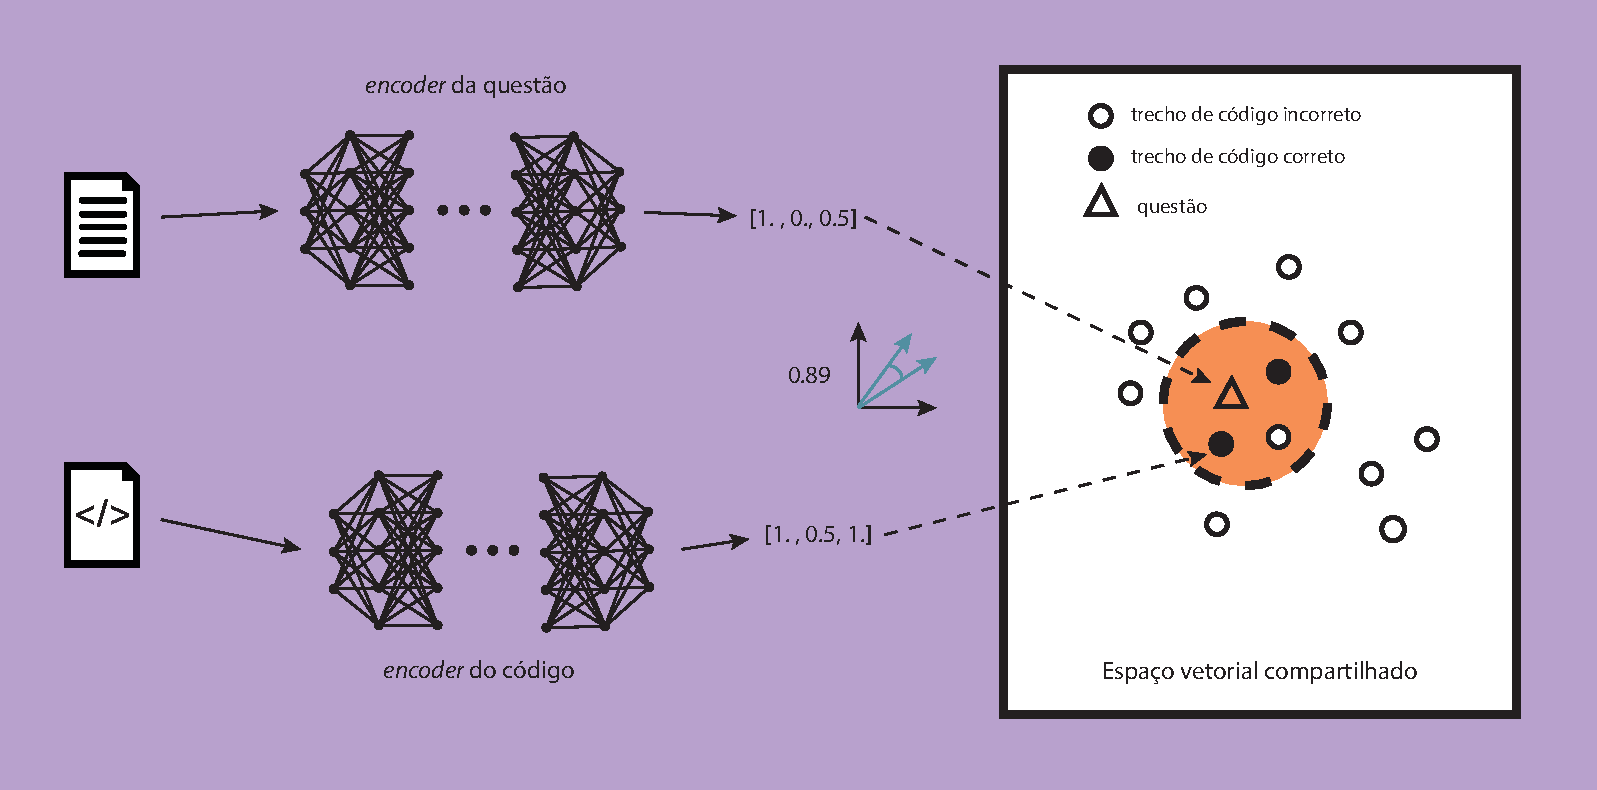
\includegraphics[width=\textwidth]{figuras/joint_embedding.pdf}
  \caption{TODO: FIX translation Illustration of \emph{joint embedding} technique for code retrieval. Two neural networks map a question and a code snippet into a common vector space. The distance between the vectors reflects the relevance of a code snippet to a question.}
  \Description{None}
  \label{fig:joint-embedding}
\end{teaserfigure}

%%
%% This command processes the author and affiliation and title
%% information and builds the first part of the formatted document.
\maketitle

\section{Introduction}

The advent of open source code and open question answering sites related to programming contributed to improve the way developers code today. Nowadays, code search is a daily routine task at software development process. Developers spend 15\% of their time searching for how a code works, a bug fix and API's usage \cite{what-developers-search-for-on-the-web:xia:2017}. According to \cite{sadowski-how-developers-search-for-code-case-study:2015}, developers at Google search for code 12 times a day, clicking on 2 to 3 results by average per search session. Most of them are looking for code examples. Thus, improve the way developers find a code it's an important productivity tool.  

Most of developers use general purpose search engine (GPSE) to look for code (e.g. Google). GPSE uses page rank and other indexes tactics that are not optimized for searching code. Then, GPSE are not capable of finding a code semantically, unless a code has a accompanying description. According to ZZZ, developers spend more time, visit more pages and change a query more times when they are searching for code compared to non-code related search.

GitHub, a popular open source code repository, have tried to build a semantic code search. They extracted millions of lines of code from his repositories and matched each code with a dosctring. The final results weren't satisfactory, the tool could find a relevant code only if the query matches the docstring description (cite HHHHHH). According to XXXXX, a user's intent were better matched with questions extracted from open question-answering sites related to programming, e.g., StackOverflow. Those sites permit users to ask a question and check the best answer for him. Other users can vote for the most helpful answer and mark wrong or not helpful ones. Those collective actions help to curate and organize information, creating a valuable repository.

There are a lot of works about semantic code search (UUUUUU). The first ones were based on deductive-logic rules and manual feature extraction from code. The recent success of artificial neural networks, due to Big Data and computational resources available, shifted works to machine learning based approach. ZZZZZ also coined a name, neural code search, i.e., code search based on neural networks.

Most of works applied neural networks to summarize and retrieve code snippets. Code summarization and retrieval are two different activities, each one with it's metric and trait. We are proposing an novel approach for code retrieval. Different from other works, which presented an neural network with attention mechanism and a recurrent neural network (RRRR, GGGG), we are proposing a code retrieval based on convolutional networks. ZZZ and YYY paired code snippets and docstring, we matched code with questions extracted from StackOverflow.

\subsection{Contributions of this work}

We can summarize the shortcomings of the existing work:
most of neural networks approaches summarize and retrieve a code, although each one has its idiosyncrasy. As far as we know, we are the first to apply convolutional neural network to code retrieval, due to good results in answer selection tasks (TTTTTT). Most of works paired code and docstring, even though docstring doesn't match user's intent. Our research are trying to address each of these in turn by proposing and analyzing the CoNCRA, \emph{a Convolutional Network Code Retrieval Approach}.

\begin{itemize}
    \item We are proposing the CoNCRA, which is motivated
by the good results of convolutional networks at Natutal Language Processing (NLP) tasks. 
    \item We paired code and questions collected from StackOverflow, based on a public available dataset (YYYY).

    \item We evaluated the efficacy of our approach against two other proposals.
    
\end{itemize}







\section{Methodology}

According to \cite{cambronero-deep-code-search-2019}, the main goal of code retrieval is:

\emph{Retrieve code snippets from a code corpus that most closely match a developer's intent, which is expressed in natural language.}

The first proposals for code search used tools based on deductive-logic rules and manual feature extraction. Deductive-logic approach, e.g. boolean model, finds a code that matches exactly the keywords expressed in the query. According to ZZZ, those approaches are good at finding API's call and error's message, but it struggles to find reusable code and examples that don't have a exactly match between the code and query. Thus, there is a need to look for a semantic code search.

Neural networks showed good results at translation, question-answering and classifications tasks in NLP, it could infer words semantic and phrases context. Then, most of recent works adopted neural networks approach. Cambronero coined a term, \emph{neural code search}, searching for code using neural networks.

The marjority of works adopted the same strategy, which is to discriminate relevant code snippets from non-relevant one's based on an user's intent. In pursuance of that, code retrieval are reduced to a ranking problem where neural networks should be able to place code snippets that closely match developer's intent in the first rank. The most common strategy to do this is \emph{joint embedding}. Joint embedding maps heterogeneous data into a common vector space, where the distance between embedded input reflects the similarity between the underlying items \cite{li-joint-embedding-images-2015} (see Figure~\ref{fig:joint-embedding}).

In order to apply joint embedding, 3 (three) items had to be considered:

\begin{itemize}
    \item Word embedding
    \item Sentence embedding
    \item Joint embedding
\end{itemize}

Embedding refers to a continuous vector in a lower dimensional vector space. A function that maps an input to a continuous vector is called \emph{encoder}. So, given an input set $X$, an encoder function $F$ can be defined as \cite{cambronero-deep-code-search-2019}:

\begin{equation}
    F: X \to E
\end{equation}

In our case, $X$ can be a set of questions or code snippets and $E$ is a set of continuous vectors or embeddings, such that $E \subset R^{d}$, where $d$ is the dimension. Our main goal is to learn two encoders $F$ and $G$ that maps a question and a code snippet, respectively, into a common vector space, so that the distance between the vectors reflect the relevance of a code snippet to a question (see Figure~\ref{fig:joint-embedding}). In our work, we are suggesting a convolutional network approach to learn the sentence embedding, i.e., a convolutional network will encode the question and code snippet into a common vector space. We also defined how words are embedded and the objective function to help neural networks to approximate questions and code snippets correctly.

\subsection{Word embedding}

The words and terms of a question and code snippet must be encoded in a numeric vector. The way those vectors are created it's very important, as a good vector will help neural networks to learn easily a task. The most common encoder for words is the \emph{word2vec}, which embeds a word in a continuous vector based on distributional hypothesis. The distributional hypothesis says two words are similar if they appear together frequently in differents contexts (cite Bengio GGGGG). Context can be a sentence, paragraph or a document in NLP tasks. In our case, it's a question and a code snippet.

Word2vec has two strategies: continuous-bag-of-words (CBoW) and skip-gram. The main difference between them is that CBoW predicts a target word given a context words and skip-gram predicts the context words given a single word. According to Mikolov BBBBB, CBoW showed good results at syntactically tasks, e.g., finding a superlative of a word or identify an adverb, while skip-gram presented a good performance at semantic tasks, e.g., finding the capital of a state or grouping feminine and masculine words. 

In our work, we opted for skip-gram as a semantic trait is preferable to a sintact one in our task. Semantic trait can help the neural network to discriminate conditional clauses (e.g. \emph{if}, \emph{elsif}) and loop iteration (e.g. \emph{for}, \emph{while}), for an example. Figure~\ref{fig:tsne-code-snippet-python} shows an application of word2vec in a Python related corpus. If we look carefully, we can see the similarities between \emph{file}, \emph{write} and \emph{open}, as \emph{set}, \emph{list} and \emph{dict} based on the distance of each one.

\begin{figure}[H]
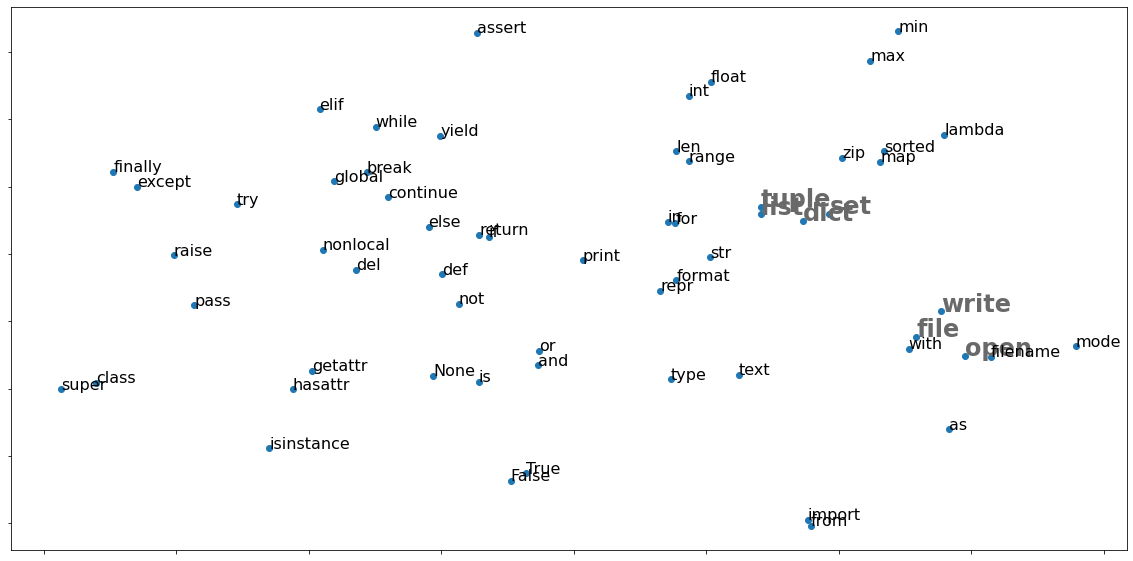
\includegraphics[width=0.45\textwidth]{figuras/code_tsne.png}
\caption{2D illustration of the continuous vectors of the 66 most common words contained in vocabulary $V$. The vocabulary $V$ contains words from questions and code snippets related to Python. The illustration was generated by t-SNE, which allows 2D visualization from high-dimensional data. We applied word2vec with skip-gram and set the parameter window to $5$.}

\label{fig:tsne-code-snippet-python}
\end{figure}

\subsection{Sentence embedding}

We can combine the word embeddings to obtain a sentence embedding. Our proposal is to combine word embeddings by using a convolutional network. Convolutional networks showed good results at answer selection task in NLP, where given a question and a set of answers, the model should rank the best answers in the firsts positions. Although, convolutional networks prioritizes local interactions (e.g. words nearby) and can't capture long range dependencies (e.g. distant words in a sentence), we think it does not represent a big problem to code retrieval, as most of questions and code snippets are short in length.

Given an sentence $\bm{x} = \{ \bm{x}(0), \bm{x}(1), . . ., \bm{x}(n - 1) \}$, such that $\bm{x}(i) \in \mathbb{R}^{d}$ is a continuous vector that represents the $i^{th}$ word of the sentence. The convolutional network combines the elements of vector $\bm{x}$ applying 3 basic operations:

\begin{itemize}
    \item Convolution operation
    \item Concatenation
    \item \textit{Maxpool}
\end{itemize}

A convolution operation uses a filter $\bm{F}  = [\bm{F}(0),· · ·, \bm{F}(m - 1)]$, such that $\bm{F} \in \mathbb{R}^{m X d}$. The operation applies the filter in $m$ words (window size) in order to produce a new vector. Suppose $\bm{x}(i, i + j)$ refer to a concatenation of the vectors $\bm{x}(i), \bm{x}(i + 1), . . ., \bm{x}(i + j)$. If we apply $\bm{F}$ to $\bm{x}(i, i + m - 1)$, then we can calculate a new vector $\bm{c}(i)$ by:

\begin{equation}\label{eq:calc_convolution_ci}
    \bm{c}(i) = tanh \left[\left(\sum_{j=0}^{m - 1} \bm{x}(i + j)^{T}\bm{F}(j)\right) + b\right]
\end{equation}

In the equation~\ref{eq:calc_convolution_ci}, $b$ is a \textit{bias} e $\bm{F}$ and $b$ are weight's filter, which will be learned by convolutional network during a training phase. The convolution operation applies ther filter $\bm{F}$ to every possible window of words using the same weight and, as a result, we have a feature map.

\begin{equation}
    \bm{c} = \{ \bm{c}(0), \bm{c}(1), . . ., \bm{c}(n - m) \} 
\end{equation}

The feature map (or activation map) contains the latent and most important features of a sentence. A convolutional network may contain thousands of filters, each one extracting specific \emph{m-gram} features. A filter of $m$ size 2 extracts bigram features, size 3 extracts trigram features and so on. The number of feature maps is $|F|$, i.e., the number of filters. After the convolution operation, a pooling layer operates independently on every feature map resizing it spatially, using a max operation \cite{karpathy-course-cnn-2016}.  The max operation is applied along the $axis=0$ to produce the final vector $\bm{o}$:

\begin{equation}
    \bm{o} = max\left(\left[\bm{c}_{1}, \bm{c}_{2}, . . ., \bm{c}_{|F|}\right], axis = 0\right)
\end{equation}

The max pooling helps the convolutional network to be translation invariant. Regardless of the word's position shift, the max pooling selects the most relevant features and insert into the final vector \citep{tom-young:trends-deep-learning-nlp}. Figure~\ref{fig:cnn-steps-word-embedding} illustrates the full operation. Our sentence embedding is the vector $\bm{o}$, so $\bm{o}$ represents a question or a code snippet, in our case. 

\begin{figure}[H]
    \centering
    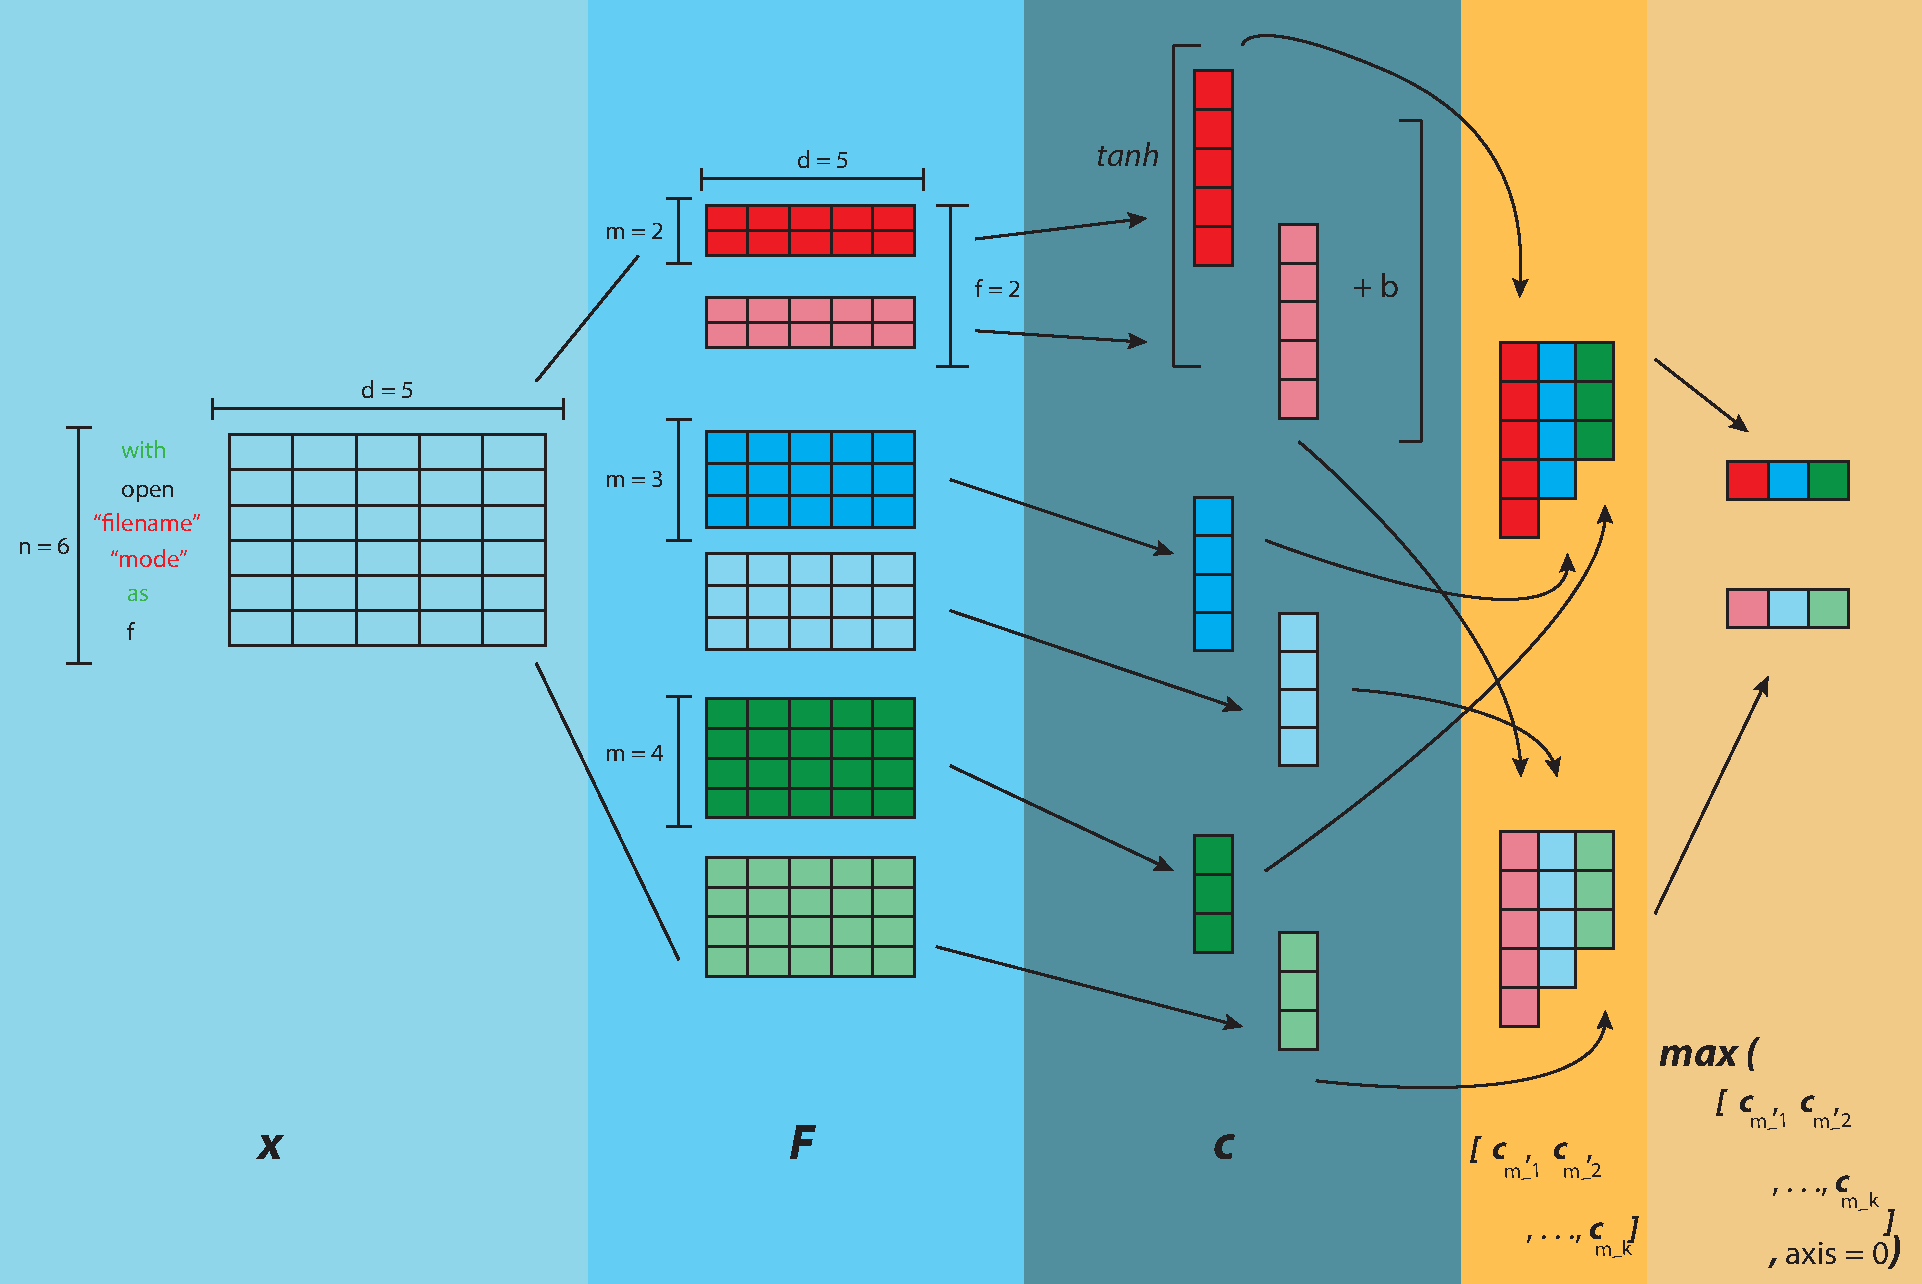
\includegraphics[width=0.45\textwidth]{figuras/cnn-steps-word-embedding.pdf}
    \caption{TO-DO: Fix image according to new equation. Ilustração das 3 operações realizadas pela nossa arquitetura CNN para obter o vetor de representação final $\bm{c'}_{\bm{m}}$. Neste exemplo, utilizamos 3 filtros $\bm{F} \in \mathbb{R}^{m X d X f}$ com diferentes janelas $m$, onde $m = \{2, 3, 4\}$. Cada filtro tem tamanho $f = 2$. Temos um total de 6 filtros ao final. Cada filtro é aplicado a sentença $\bm{x} \in \mathbb{R}^{n X d}$, onde $n = 6$ e $d = 5$. O primeiro passo é a obtenção do vetor $\bm{c}$ de características. Posteriormente, é realização a operação de concatenação, no qual é obtido o vetor $\bm{c}_{\bm{m}}$, conforme descrito na operação~\ref{eq:concatenacao-cnn-cm}. Ao final, a operação \textit{max} é aplicada no eixo $0$, obtendo o vetor de representação final $\bm{c'}_{m}$. Este vetor $\bm{c'}_{m}$ será o nosso vetor de representação das nossas sentenças, i.e., o vetor de representação das questões e trechos de código-fonte. Figura adaptada do artigo de \cite{zhang-guide-convolutional-cnn-embedding-ilustration:2015}}
    \label{fig:cnn-steps-word-embedding}
\end{figure}

\subsection{Joint embedding}

In our work, we reduced code retrieval to a ranking problem, where a model should rank a relevant code in the firsts positions based on a developer's intent. In order to do that, we choose an objective function that prioritizes the relative preference of the code snippets, instead of a correct classification. The objective function, in our case, helps the neural network to discriminate the correct answers from incorrect ones during the training phase.


Given a question and code snippet set, $\mathbb{Q}$ and $\mathbb{C}$ respectively, our training input is composed by a triple $<\bm{q}, \bm{c^{+}}, \bm{c^{-}}>$, where $\bm{c^{+}} \in \mathbb{C}$ indicates a correct code snippet for a question $\bm{q} \in \mathbb{Q}$ and $\bm{c^{-}} \in \mathbb{C}$ its an incorret one sampled from the training data. We used the hinge loss as our objective function. Formally, for a triple $<\bm{q}, \bm{c^{+}}, \bm{c^{-}}>$, the definition of hinge loss is:

\begin{equation}
J = max(0, m - h_{\theta}(\bm{q}, \bm{c^{+}}) + h_{\theta}(\bm{q}, \bm{c^{-}}))
\end{equation}

$m$ its a margin and $h_{\theta}$ its a similarity function (e.g., \textit{cosine}). During the training phase, the goal is to minimize the cost function $J$. In order to obtain that, the model aims to satisfy the following condition: $h_{\theta}(\bm{q}, \bm{c^{+}}) - h_{\theta}(\bm{q}, \bm{c^{-}}) \geq m$. Then, the hinge loss function induces our model to score $c^{+}$ higher than $c^{-}$ for a given margin $m$. 

For the similarity function $h_{\theta}$, we used \emph{cosine}, such that $h_{\theta}(\bm{q}, \bm{c}) = \{h_{\theta}(\bm{q}, \bm{c}) \in \mathbb{R} | 0 \leq h_{\theta}(\bm{q}, \bm{c}) \leq 1$\} computes the similarity between the vector $\bm{q} \in \mathbb{Q}$ and $\bm{c} \in \mathbb{C}$, where $0$ indicate orthogonality e $1$ indicate greater similarity (citar keras documentacao).  Given that our objective function aims to satisfy the following condition: $h_{\theta}(\bm{q}, \bm{c^{+}}) \geq h_{\theta}(\bm{q}, \bm{c^{-}}) + m$. Thus, we are inducing our model to group $\bm{c^{+}}$ and $\bm{q}$ nearby, while the vectors $\bm{c^{-}}$ are far away (see Figure~\ref{fig:joint-embedding}). 

\section{Experiments}

We evaluated our proposed approach (CoNCRA) on StaQC dataset, a systematically mined question code dataset from StackOverflow (citar Yang...). The main difference of StaQC to other datasets (citar referencias TTT) is it is composed by ''how-to-do-it'' questions, as the answers to those type of questions are more straight. StaQC contains SQL and Python question and code pairs, but, in our preliminary experiment, we used the python ones only. Table~\ref{table:summary-training-data-yao-staqc} gives an overview about StaQC dataset.

\begin{table}[h]
\centering
\begin{tabular}{ p{16em} P{10em} P{10em} }
\hline
  & \multicolumn{2}{c}{\textbf{Questão}}\\
\hline
\textbf{Código-fonte} & \textbf{Python} & \textbf{SQL}  \\
\hline

$N_{1}$: Apenas 1 trecho de código na descrição da resposta & $85.294$ & $75.637$ \\

$N_{2}$: Trechos de código-fonte anotados automaticamente & $60.083$ & $41.826$ \\

$N_{3}$: Trechos de código-fonte anotados manualmente & $2.169$ & $2.056$  \\

 \hline
 \textbf{Total} & $\bm{147.546}$ & $\bm{119.519}$\\
 \hline 
 
\end{tabular}
\caption{Divisão do conjunto de dados disponibilizado por \cite{yao-2018}. O conjunto formado por "Trechos de código-fonte anotados automaticamente" contém questões que tem mais de um trecho de código-fonte por resposta. Quando há mais de um trecho de código-fonte na descrição da resposta, pode haver algum trecho que não seja solução. Nesse caso, \cite{yao-2018} criaram um framework para anotá-los automaticamente e obtiveram F1 de $0,916$ e acurácia de $0,911$ em seus resultados de classificação automática das respostas corretas.}
\label{table:summary-training-data-yao-staqc}
\end{table}

\begin{table}[h]
\centering
\begin{tabular}{ l r  }
 \hline
 \textbf{Amostras} & \textbf{Quantidade de pares $<q_{i}, c_{i}^{+}>$}\\
 \hline
 $N_{2} = \text{Treinamento}$ & $60.083$\\
 
 $N_{3} \supset \text{DEV}$ & $1.085$ \\
 
 $N_{3} \supset \text{EVAL}$ & $1.084$\\
 \hline
 \textbf{Total} & $\bm{62.252}$\\
 \hline
\end{tabular}
\caption{Divisão das amostras para treinamento e avaliação. O conjunto de dados é formado por pares $<q_{i}, c_{i}^{+}>$, onde $q_{i}$ é uma questão e $c_{i}^{+}$ é um trecho de código-fonte anotado como correto. O conjunto formado por pares anotados manualmente foi dividido em DEV e EVAL conforme o procedimento descrito por \cite{iyer-etal-2016-summarizing}. É possível visualizar uma ilustração deste procedimento nas Figuras \ref{fig:evaluation-process} e \ref{fig:final-evaluation-process}.}
\label{table:training-sample-division}
\end{table}

We trained our model on sample $N2$ (see Table~\ref{table:summary-training-data-yao-staqc} and Table~\ref{table:training-sample-division}), because 27\% of the questions contains more than one answer annotated, leading to more variance in our training dataset. The training and evaluation follows the Iyer XXXX procedure, where the model is evaluated on an manually annotated dataset each epoch based on mean reciprocal rank (MRR). The MRR tells if your model ranked the annotated answer in higher positions or not, higher values indicates the accepted answers were ranked in the firts positions.

For the training phase, we used 70\% of $N2$ sample for training and 30\% for validation. The models runs during 500 epochs and stops early if the training loss ($J$) is less than $0.0001$ or the validation loss doesn't improve after 25 consecutive epoches. We choose the best model of the training phase according to MRR and run it 20 times in the $N3$ sample for the final evaluation (see Table~\ref{table:training-sample-division}). The final result is the average of the MRR for each pair $<q_{i}, c_{i}^{+}>$ of $N3$ and other 49 distractors $c_{j}$, selected randomly from the training sample, such that $c_{i}^{+} \neq c_{j}$.

 We provided the source code for our preliminary experiments in the following repository: \url{https://github.com/mrezende/concra}. The repository contains our proposed model, the baseline models, training and evaluation source code. We also provided the original and pre-processed dataset. The source code is written in Python, version 3.6.9, and we used the libraries Keras (version 2.2.4-tf) and Tensorflow (1.15.2). The preliminary experiments were all conducted in the Colab, a Google platform that allows to run arbitrary python code from the browser and it's specially suited for machine learning and data analysis research.

\subsection{Results}
Avaliamos a arquitetura CNN juntamente com outras duas arquiteturas, Embedding e \Gls{unif} na recuperação de trecho de código-fonte através do procedimento proposto por \cite{iyer-etal-2016-summarizing} e descrito na Seção~\ref{sec:avaliacao}. Os resultados foram coletados a partir da amostra \emph{EVAL} e o valor final MRR é a média obtida após 20 iterações. Conforme a Tabela~\ref{table:resultados}, as arquiteturas CNNs compartilhadas com 4000 filtros convolucionais (linhas D3 e F3) obtiveram o melhor resultado. A arquitetura CNN obteve uma média MRR 5\% superior ao melhor resultado obtido pela arquitetura Unif (linha B1), atual estado da arte, e um resultado 11\% superior a arquitetura de referência Embedding (linha A1). 

\begin{table*}[t]
\centering
\begin{tabular}{ p{1cm} p{6cm} >{\raggedleft\arraybackslash}p{4cm} >{\raggedleft\arraybackslash}p{4cm} }
 \hline
    & & \multicolumn{2}{c}{\textbf{Resultados}}\\
 \hline
 & \textbf{Modelos} & \textbf{MRR} & \textbf{TOP1}\\
 \hline
 A1 & Embedding (m = $0.1$) & $0.637$& $0.493 \pm 0.009$\\
 
 \hline
 
 B1 & Unif (m = $0.2$) & $0.675 \pm 0.006$ & $0.539 \pm 0.009$\\
 
 \hline
 
 C1 & CNN / F = 1000 & $0.669 \pm 0.006$ & $0.527 \pm 0.012$\\
 
 C2 & CNN / F = 2000 & $0.673 \pm 0.007$ & $0.531 \pm 0.012$\\
 
 C3 & CNN / F = 4000 & $0.687 \pm 0.006$ & $0.553 \pm 0.011$\\
 
 \hline
 
 D1 & CNN Compartilhado / F = 1000 & $0.678 \pm 0.007$ & $0.548 \pm 0.012$\\
 
 D2 & CNN Compartilhado / F = 2000 & $0.694 \pm 0.008$ & $0.565 \pm 0.012$\\
 
 D3 & CNN Compartilhado / F = 4000 & $0.700 \pm 0.004$ & $0.569 \pm 0.009$\\
 
 \hline
 
 E1 & CNN com NL / F = 1000 & $0.682 \pm 0.007$ & $0.543 \pm 0.012$\\
 
 E2 & CNN com NL / F = 2000 & $0.689 \pm 0.006$ & $0.553 \pm 0.011$\\
 
 E3 & CNN com NL / F = 4000 & $0.688 \pm 0.006$ & $0.553 \pm 0.011$\\
 
 \hline
 
 F1 & CNN Compartilhado com NL / F = 1000 & $0.690 \pm 0.008$ & $0.553 \pm 0.015$\\
 
 F2 & CNN Compartilhado com NL / F = 2000 & $0.700 \pm 0.007$ & $0.573 \pm 0.012$\\
 
 F3 & CNN Compartilhado com NL / F = 4000 & $0.701 \pm 0.008$ & $0.577 \pm 0.015$\\
 
\hline
\end{tabular}
\caption{Resultado do modelo CNN em comparação com as outras arquiteturas unif e Embedding. MRR refere-se a média do resultado do Mean Reciprocal Rank na amostra EVAL. TOP1 refere-se a frequência da ocorrência da resposta anotada como correta na primeira posição em comparação com outros 49 distratores. Nas linhas A1 e B1, \emph{m} refere-se ao hiper-parâmetro margem utilizada na função de perda \emph{hinge}. F indica a quantidade de filtros convolucionais utilizados durante o treinamento das redes convolucionais. NL é o acrônimo de normalização em lote. As arquiteturas CNN utilizaram margem $m = 0.05$ e o tamanho da janela do filtro (kernel) $k = 2$.}
\label{table:resultados}
\end{table*}

Conforme os resultados da Tabela~\ref{table:resultados}, os ajustes dos hiper-parâmetros para a arquitetura CNN foram ao encontro de \cite{tan-lstm-qa, feng-2015}, no qual verificaram que o aumento da quantidade de filtros convolucionais, que aumenta a capacidade das redes convolucionais e as características latentes a serem extraídas, resultaram em uma melhora no desempenho do modelo (linhas D3 e F3). Além disso, verificamos que o valor $2$ para o tamanho da janela dos filtros obteve os melhores resultados, não havendo melhora significativa para janelas de tamanho $3$ ou $4$. E diferentemente do apontamento feito por \cite{tang-hybrid-deep-representation-2018}, não notamos melhora no desempenho através da combinação de filtros com janelas de tamanhos diferentes, e.g., $2,3,5,7$ (ver Apêndice~\ref{ape:ajuste-hiper-parametros-cnn}). Porém com relação a margem utilizada na função de perda hinge, as redes convolucionais obtiveram um resultado melhor com $0.05$, já Unif obteve o melhor resultado com $0.2$ e enquanto Embedding obteve com $0.1$ (ver Apêndice~\ref{ape:ajuste-hiper-parametros-cnn}). No caso de \cite{tan-lstm-qa} ele fixou a margem em $0.2$. Em nosso caso, preferimos fixar valores diferentes de margem para cada arquitetura, pois conforme os experimentos descritos no Apêndice~\ref{ape:ajuste-hiper-parametros-cnn}, diferentes valores de margem levaram a diferentes desempenhos do modelo. E segundo \cite{park-regarding-margin-loss:2017}, nem sempre os valores mais altos para a margem levam a um melhor desempenho do modelo, por isso faz-se necessário o ajuste do parâmetro da função de perda \textit{hinge} também. 


Conforme verificado por \cite{tan-lstm-qa} e \cite{feng-2015}, as redes convolucionais que compartilham os parâmetros dos pares de questões e respostas durante a aprendizagem (linhas D e F) obtiveram um desempenho superior aos modelos que utilizaram parâmetros independentes (linhas C e E). De acordo com \cite{tan-lstm-qa}, os parâmetros indepdendentes tornam a aprendizagem mais difícil, pois o otimizador terá que aprender o dobro de parâmetros. Já para \cite{wen-joint-modeling-question-answer-2019}, as redes convolucionais que aprendem as representações de forma independente e postergam a interação entre elas para a última camada (cálculo da similaridade e função de perda \textit{hinge}), exploram de forma ineficiente a correlação semântica entre as respectivas representações dos pares de questões e respostas. No nosso caso, verificamos que ao treinar por mais épocas, não houve melhora significativa no desempenho, salientando a dificuldade das redes convolucionais que aprendem as representações de forma independente em encontrar uma correlação semântica entre os pares de questões e respostas.

Durante o treinamento, para evitar o \textit{overfitting} dos modelos, adotamos a técnica de normalização em lote, que além de melhorar o desempenho, a velocidade e a estabilidade das redes neurais, ele mitiga o \textit{overfitting}, reduzindo a necessidade do uso de outra técnica de regularização como o \textit{dropout} \citep{sergey-batch-normalization-2015}. No nosso caso, verificamos a melhora no desempenho e robustez das redes convolucionais (ver linhas E e F da Tabela~\ref{table:resultados} e ver Apêndice~\ref{ape:ajuste-hiper-parametros-cnn}). No caso da arquitetura Unif, optamos por manter a arquitetura padrão proposta por \cite{cambronero-deep-learning-code-search:2019}. E a arquitetura \textit{Embedding}, por ser mais simples e ter apenas uma camada de \textit{maxpool}, não teve a necessidade de regularização.


Para entender um pouco melhor o resultado da média harmônica MRR, a Figura~\ref{fig:histogram-mrr} exibe as posições da primeira ocorrência do trecho de código-fonte encontradas durante a avaliação dos modelos.

\begin{figure}[H]
    \centering
    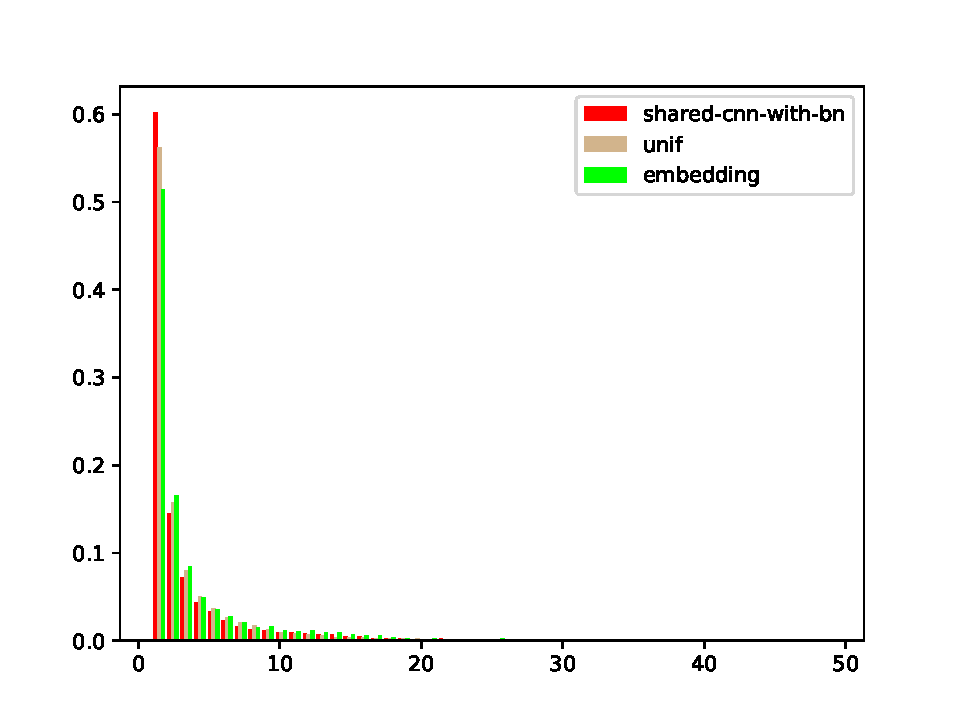
\includegraphics[width=0.45\textwidth]{figuras/histogram.pdf}
    \caption{Figura das primeiras posições observadas para o trecho de código-fonte anotado como correto. As legendas \emph{shared-cnn-with-bn}, \emph{unif} e \emph{embedding} referem-se as linhas F3, A1 e B1 da Tabela~\ref{table:resultados} respectivamente.}
    \label{fig:histogram-mrr}
\end{figure}


Tanto o CNN quanto a arquitetura Unif conseguiram classificar os trechos de código-fonte entre as 3 (três) primeiras posições em 75\% dos casos. A nossa arquitetura proposta obteve uma precisão TOP-1 de aproximadamente 60\%, i.e., em aproximadamente 60\% das vezes, o trecho de código-fonte relevante ficou na primeira posição. Já a arquitetura Unif e Embedding obtiveram uma precisão TOP-1 de pouco mais de 50\%. Um ponto a ser levantado é que a nossa métrica MRR só leva em consideração a posição apontada pelo modelo para o trecho de código-fonte anotado como correto. Mesmo que o modelo apresente um outro trecho de código-fonte que também é solução, o nosso método de avaliação não leva em consideração. Neste caso, o modelo é penalizado.

\subsection{Threats to validity}

Conforme citado anteriormente, \cite{yao-2018} anotaram o conjunto de dados utilizando um framework proposto em seu artigo. Para anotá-los, os autores treinaram uma rede neural no conjunto de dados anotado manualmente. Em nosso trabalho, fizemos o caminho inverso. Treinamos os nossos modelos nos dados anotados automaticamente e avaliamos no conjunto anotado manualmente. Para diminuir o viés, adotamos o procedimento proposto por \cite{iyer-etal-2016-summarizing} descrito na Seções~\ref{sec:treinamento} e \ref{sec:avaliacao}.

\section{Related Work}

\section{Conclusion}

\section{Acknowledgments}

Identification of funding sources and other support, and thanks to
individuals and groups that assisted in the research and the
preparation of the work should be included in an acknowledgment
section, which is placed just before the reference section in your
document.

This section has a special environment:
\begin{verbatim}
  \begin{acks}
  ...
  \end{acks}
\end{verbatim}
so that the information contained therein can be more easily collected
during the article metadata extraction phase, and to ensure
consistency in the spelling of the section heading.

Authors should not prepare this section as a numbered or unnumbered {\verb|\section|}; please use the ``{\verb|acks|}'' environment.

\section{Appendices}

If your work needs an appendix, add it before the
``\verb|\end{document}|'' command at the conclusion of your source
document.

Start the appendix with the ``\verb|appendix|'' command:
\begin{verbatim}
  \appendix
\end{verbatim}
and note that in the appendix, sections are lettered, not
numbered. This document has two appendices, demonstrating the section
and subsection identification method.

\section{SIGCHI Extended Abstracts}

The ``\verb|sigchi-a|'' template style (available only in \LaTeX\ and
not in Word) produces a landscape-orientation formatted article, with
a wide left margin. Three environments are available for use with the
``\verb|sigchi-a|'' template style, and produce formatted output in
the margin:
\begin{itemize}
\item {\verb|sidebar|}:  Place formatted text in the margin.
\item {\verb|marginfigure|}: Place a figure in the margin.
\item {\verb|margintable|}: Place a table in the margin.
\end{itemize}

%%
%% The acknowledgments section is defined using the "acks" environment
%% (and NOT an unnumbered section). This ensures the proper
%% identification of the section in the article metadata, and the
%% consistent spelling of the heading.
\begin{acks}
To Robert, for the bagels and explaining CMYK and color spaces.
\end{acks}

%%
%% The next two lines define the bibliography style to be used, and
%% the bibliography file.
\bibliographystyle{ACM-Reference-Format}
\bibliography{sample-base}

%%
%% If your work has an appendix, this is the place to put it.
\appendix

\section{Research Methods}

\subsection{Part One}

Lorem ipsum dolor sit amet, consectetur adipiscing elit. Morbi
malesuada, quam in pulvinar varius, metus nunc fermentum urna, id
sollicitudin purus odio sit amet enim. Aliquam ullamcorper eu ipsum
vel mollis. Curabitur quis dictum nisl. Phasellus vel semper risus, et
lacinia dolor. Integer ultricies commodo sem nec semper.

\subsection{Part Two}

Etiam commodo feugiat nisl pulvinar pellentesque. Etiam auctor sodales
ligula, non varius nibh pulvinar semper. Suspendisse nec lectus non
ipsum convallis congue hendrerit vitae sapien. Donec at laoreet
eros. Vivamus non purus placerat, scelerisque diam eu, cursus
ante. Etiam aliquam tortor auctor efficitur mattis.

\section{Online Resources}

Nam id fermentum dui. Suspendisse sagittis tortor a nulla mollis, in
pulvinar ex pretium. Sed interdum orci quis metus euismod, et sagittis
enim maximus. Vestibulum gravida massa ut felis suscipit
congue. Quisque mattis elit a risus ultrices commodo venenatis eget
dui. Etiam sagittis eleifend elementum.

Nam interdum magna at lectus dignissim, ac dignissim lorem
rhoncus. Maecenas eu arcu ac neque placerat aliquam. Nunc pulvinar
massa et mattis lacinia.

\end{document}
\endinput
%%
%% End of file `sample-sigconf.tex'.
